\tikzset{
            logicalcnot/.pic = {
                \node at (-1, -4.75) {$CNOT_L$};
                
                {
                    
                    \draw[color=black, thin] (-2, -2.75) -- (0, -2.75);
                    \draw[color=black, fill=black, thick] (-1, -2.75) circle (0.1);
                    
                    
                    \draw[color=black, thin] (-1, -3.75) -- (-1, -2.75);
                    
                    
                    \draw[color=black, thin] (-2, -3.75) -- (0, -3.75);
                    \node at (-1, -3.75) {\Large $\oplus$};
                }
                
                
                \draw[color=black, thin] (2, 0.5) -- (7, 0.5);
                \draw[color=black, fill=black, thick] (2.4,0.5) circle (0.1);
                
                
                \draw[color=black, thin] (2, 0) -- (7, 0);
                \draw[color=black, fill=black, thick] (3.1, 0) circle (0.1);

                
                \draw[color=black, thin] (2, -0.5) -- (7, -0.5);
                \draw[color=black, fill=black, thick] (3.8, -0.5) circle (0.1);

                
                \draw[color=black, thin] (2, -1) -- (7, -1);
                \draw[color=black, fill=black, thick] (4.5, -1) circle (0.1);

                
                \draw[color=black, thin] (2, -1.5) -- (7, -1.5);
                \draw[color=black, fill=black, thick] (5.2, -1.5) circle (0.1);

                
                \draw[color=black, thin] (2, -2) -- (7, -2);
                \draw[color=black, fill=black, thick] (5.9, -2) circle (0.1);

            
                
                \draw[color=black, thin] (2, -2.5) -- (7, -2.5);
                \draw[color=black, fill=black, thick] (6.6, -2.5) circle (0.1);

                
                \draw[color=black, thin] (2.4, 0.5) -- (2.4, -4);
                \draw[color=black, thin] (3.1, 0) -- (3.1, -4.5);
                \draw[color=black, thin] (3.8, -0.5) -- (3.8, -5);
                \draw[color=black, thin] (4.5, -1) -- (4.5, -5.5);
                \draw[color=black, thin] (5.2, -1.5) -- (5.2, -6);
                \draw[color=black, thin] (5.9, -2) -- (5.9, -6.5);
                \draw[color=black, thin] (6.6, -2.5) -- (6.6, -7);

                
                
                \draw[color=black, thin] (2, -4) -- (7, -4);
                \node at (2.4, -4) {\Large $\oplus$};
                
                
                \draw[color=black, thin] (2, -4.5) -- (7, -4.5);
                \node at (3.1, -4.5) {\Large $\oplus$};

                
                \draw[color=black, thin] (2, -5) -- (7, -5);
                \node at (3.8, -5) {\Large $\oplus$};

                
                \draw[color=black, thin] (2, -5.5) -- (7, -5.5);
                \node at (4.5, -5.5) {\Large $\oplus$};

                
                \draw[color=black, thin] (2, -6) -- (7, -6);
                \node at (5.2, -6) {\Large $\oplus$};

                
                \draw[color=black, thin] (2, -6.5) -- (7, -6.5);
                \node at (5.9, -6.5) {\Large $\oplus$};

                
                \draw[color=black, thin] (2, -7) -- (7, -7);
                \node at (6.6, -7) {\Large $\oplus$};

                
                \draw[thick, -latex](0.5, -3.25) -- (1.5, -3.25);
            }
        }
\begin{figure*}
    \begin{minipage}[c]{0.6\textwidth}
        \centering
        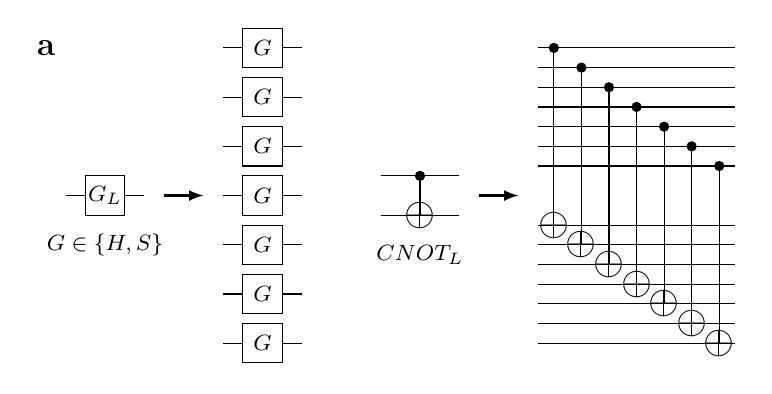
\begin{tikzpicture}[scale=0.5,font={\footnotesize}]
            \node at (-2.5, 0.5) {\large \textbf{a}};

            \node at (-1, -4.5) {$G \in \{H,S\}$};
            \draw[color=black, thin] (-2, -3.25) -- (0, -3.25);
            \draw[color=black, fill=white, thin] (-1.5, -3.75) rectangle (-0.5,-2.75) node[midway] {$G_{L}$};
            
            
            \draw[color=black, thin] (2, 0.5) -- (4, 0.5);
            \draw[color=black, fill=white, thin] (2.5,0) rectangle (3.5,1) node[midway] {$G$};

            
            \draw[color=black, thin] (2, -0.75) -- (4, -0.75);
            \draw[color=black, fill=white, thin] (2.5,-1.25) rectangle (3.5,-0.25) node[midway] {$G$};
            
            
            \draw[color=black, thin] (2, -2) -- (4, -2);
            \draw[color=black, fill=white, thin] (2.5,-2.5) rectangle (3.5,-1.5) node[midway] {$G$};
            
            
            \draw[color=black, thin] (2, -3.25) -- (4, -3.25);
            \draw[color=black, fill=white, thin] (2.5,-3.75) rectangle (3.5,-2.75) node[midway] {$G$};

            
            \draw[color=black, thin] (2, -4.5) -- (4, -4.5);
            \draw[color=black, fill=white, thin] (2.5,-5) rectangle (3.5,-4) node[midway] {$G$};

            
            \draw[color=black, thin] (2, -5.75) -- (4, -5.75);
            \draw[color=black, fill=white, thin] (2.5,-6.25) rectangle (3.5,-5.25) node[midway] {$G$};

            
            \draw[color=black, thin] (2, -7) -- (4, -7);
            \draw[color=black, fill=white, thin] (2.5,-7.5) rectangle (3.5,-6.5) node[midway] {$G$};

            
            \draw[thick, -latex](0.5, -3.25) -- (1.5, -3.25);

            \pic[scale=0.5] at (8, 0) {logicalcnot};
        \end{tikzpicture}
    \end{minipage}
    \begin{minipage}{0.3\textwidth}
        \centering
        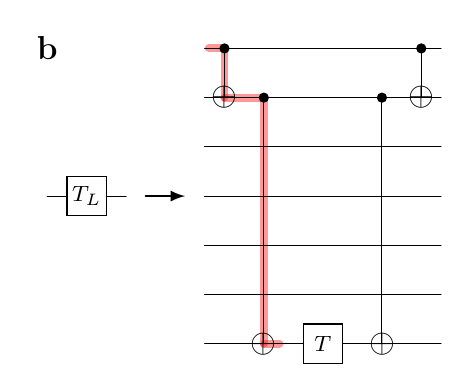
\begin{tikzpicture}[scale=0.5,font={\footnotesize},line cap=round]
            \node at (-4, 0.5) {\large \textbf{b}};

            \draw[color=black, thin] (-4, -3.25) -- (-2, -3.25);
            \draw[color=black, fill=white, thin] (-3.5, -3.75) rectangle (-2.5,-2.75) node[midway] {$T_{L}$};
            
            
            \draw[thick, -latex](-1.5, -3.25) -- (-0.5, -3.25);

            
            \draw[color=red, line width=1mm, opacity=0.4] (0.1, 0.5) -- (0.5, 0.5);
            \draw[color=red, line width=1mm, opacity=0.4] (0.5, 0.5) -- (0.5, -0.75);
            \draw[color=red, line width=1mm, opacity=0.4] (0.5, -0.75) -- (1.5, -0.75);
            \draw[color=red, line width=1mm, opacity=0.4] (1.5, -0.75) -- (1.5, -7);
            \draw[color=red, line width=1mm, opacity=0.4] (1.5, -7) -- (1.9, -7);


            \draw[thin](0, 0.5) -- (6, 0.5);
            \draw[thin](0, -0.75) -- (6, -0.75);
            \draw[thin](0, -2) -- (6, -2);
            \draw[thin](0, -3.25) -- (6, -3.25);
            \draw[thin](0, -4.5) -- (6, -4.5);
            \draw[thin](0, -5.75) -- (6, -5.75);
            \draw[thin](0, -7) -- (6, -7);

            \draw[color=black, fill=black, thick] (0.5, 0.5) circle (0.1);
            \draw[color=black, fill=black, thick] (1.5, -0.75) circle (0.1);
            \draw[color=black, fill=black, thick] (5.5, 0.5) circle (0.1);
            \draw[color=black, fill=black, thick] (4.5, -0.75) circle (0.1);

            \draw[color=black, thin] (0.5, 0.5) -- (0.5, -0.75);
            \draw[color=black, thin] (1.5, -0.75) -- (1.5, -7);
            \draw[color=black, thin] (4.5, -0.75) -- (4.5, -7);
            \draw[color=black, thin] (5.5, 0.5) -- (5.5, -0.75);

            \node at (0.5, -0.75) {\large$\displaystyle\oplus$};
            \node at (1.5, -7) {\large$\displaystyle\oplus$};
            
            \node at (5.5, -0.75) {\large$\displaystyle\oplus$};
            \node at (4.5, -7) {\large$\displaystyle\oplus$};


            \filldraw[color=black, fill=white, thin] (2.5,-7.5) rectangle (3.5,-6.5) node[midway] {$T$};
        \end{tikzpicture}
    \end{minipage}
    \caption{\textbf{a)} Transversal implementation of the logical Clifford gates for the Steane code. The logical $H_L$ and $S_L$ gates are trivially transversal because the physical gates act on each qubit individually. For the logical $CNOT_L$ notice that the $i$th qubit of the first block of seven qubits only interacts with the $i$th qubit of the second block. \textbf{b)} Non-transversal implementation of the $T$ gate for the Steane code. The red line indicates the propagation of a single-qubit error to three different qubits.}\label{fig:steane-logical-gates}
\end{figure*}